%%% mrw.tex
%%% from spire2024 sub

\section{A Modified Algorithm for Minimal Rare Words}
\label{sec:mrw}

%%%%%%%%%%%%%%
%\paragraph{Algorithms for MRW}
In this section, we present a modified algorithm for computing $\MRWK[k]$ with any $k\ge 1$. 
We start with a characterization of $\MRWS[\ge k](S) := \bigcup_{k\ge 1}\MRWK[k]$ in maximal repeats in $\MR$. 
Suppose that $|S|\ge 2$ and $|\Sigma(S)|\ge 2$
The next lemma is a slightly modified version of the result shown by Belazzougui and Cunial~\cite{belazzougui2015space:unusual}. For the completeness, we show a sketch of the proof. 

\begin{lemma}[characterization of $\MRW_k(S)$~\cite{belazzougui2015space:unusual}]\label{lem:characterization:mrw}
For any $k\ge 0$, any $a, b \in \Sigma$, and $u\in\Sigma^*$, the conditions (1) and (2) are equivalent: 
\begin{enumerate*}[(1)]
\item $W = aub \in \MRWK[k]$. 
\item $u\in\MR(S)$, $|\RSigma[](au)| \ge 2$, $|\LSigma[](ub)| \ge 2$, and $\Occ[](aub) = k$. 
\end{enumerate*}
\end{lemma}

\begin{proof}
  (1) $\Rightarrow$ (2):  Suppose that $aub \in \MRWK[k]$ holds. From defininition, $\Occ[](aub) = k$ follows. By contradiction, suppose that $|\RSigma[](au)| = 1$. If we let $\RSigma[](au) = \set{c}$ for a character $c \in \Sigma$, it follows that $\Occ[](au) = \Occ[](aub) = k$, contradiction. Therefore, we have $|\RSigma[](au)| \ge 2$. Since $|\RSigma[](u)| \ge |\RSigma[](au)| \ge 2$, we see that $u$ is right-branching. By symmetry, we can also show that $|\LSigma[](ub)| \ge 2$, and thus, $u$ is left-branching. Combining the arguments, we conclude that $u \in \MR(S)$.
  %%% 
 (2) $\Rightarrow$ (1):  Suppose that $\Occ[](aub) = k$. 
  If $|\RSigma[](au)| \ge 2$ and character $b$ is contained in $\RSigma[](au)$, then we have $\Occ[](au) > \Occ[](aub) = k$. By symmetry, if $|\RSigma[](au)| \ge 2$, then $\Occ[](ub) > \Occ[](aub) = k$ follows. Combining the above arguments, the claim is proved. 
\qed\end{proof}



%%%%%%%%%%%%%%%%%%%%%%%%%%%%
\begin{algorithm}[t]
  \caption{A fragment of the code for a modified algorithm for enumerating the set $\MRWK[\ge 1](S)$ of all minimal rare words of a string $S$ over alphabet $\Sigma$.
}\label{fig:example:mrw:subcode}
%%%\medskip
  \KwInput{
    A triple $\pair{i..j, \ell} \in \RREP$,
    a monotone constraint $\Theta \subseteq \Sigma^*$, and 
    a set $Words \subseteq \RREP$. 
  }
  %% \KwOutput{
  %%   the set $\MR(S)$ of all maximal reepeats of the string $S$ prefixed by the word $u := \getfactor(i..j, \ell)$. 
  %% }
  %% \textbf{procedure} \MRRec$(\pair{i..j, \ell}, \Theta, Words)$\;
  %% \Begin{
  %%     %\textbf{output} $(i..j, \ell)$
  %%     \If{$u := \getfactor(i..j, \ell) \not\in \Theta$}{
  %%       \Return $Words$\; 
  %%     }
  %%     $Words.\append(\pair{i..j, \ell})$
  %%     \Comment*{A maximal repeat is found}
  %%     $Children \gets \emptyset$\; 
  %%     $Children \gets \GenChildren(i..j, \ell, Children)$\Comment*{See \cref{lem:genchildren}}
  \Begin{
      $Children \gets \GenChildren(i..j, \ell, Children)$\; 
      \For {each child $(b, \pair{i_b..j_b, \ell_b}) \in Children$}{
            \Comment{The triple represents a factor $w_b = \getfactor(i_b..j_b, \ell_b)$ as a child of $u$}
             %% \Comment{Postcondition:
             %%   $b \in \LSigma[](\getfactor(i..j, \ell))$ and 
             %%   the factor $u_b = \getfactor(i_b..j_b, \ell_b)$
             %%   is a repeat with $|\LSigma[](u_b)| \ge 2$.                
             %% }
            \If (\comblk{See \cref{lem:leftmaximal:character}}) {$\isLeftBranching(i_b..j_b, \ell_b)$}{
              \Comment{Computing the set of left characters $L_b = \LSigma[](w_b)= \LSigma[](ub)$}
              %% $L_0 \gets \ColoredRange(i, j)$\; 
              $L_b \gets \ColoredRange(i_b, j_b)$\;
              \For{each $(a, k_{ab}) \in L_b$}{
                \Comment{Notes: the character $a$ is a member of $\LSigma[](u)$ and $k_{ab} \ge 1$ is the frequency of $a$ in the range $\BWT[i_b..j_b]$.}
                Compute the range $i_{ab}..j_{ab}$ of factor $aub$ from $i_b..j_b$ based on the LF-mapping\; 
                $Words[k_{ab}].\append(\pair{i_{ab}..j_{ab}, \ell+2})$ \Comment*{the triple for $aub$}
              }
              $Words \gets \MRRec(\pair{i_b..j_b, \ell_b}, \Theta, Words)$\;
          } %% if 
       } %% for 
   }%% Begin
\end{algorithm}
%%%%%%%%%%%%%%%%%%%%%%%%%%%%


  Fromn \cref{lem:characterization:mrw},
  we show in Algorithm~\ref{fig:example:mrw:subcode} the modified code for enumeration of $\MRWK[\ge 1]$, which will be substituted for the for-loop from \ref{line:recmr:for:begin} to \ref{line:recmr:for:end} in the body of the recursive subprocedure $\MRRec$ in Algorithm~\ref{fig:example:mrep:sub}.
  Using the modified algorithm, we can show the main result of this section. 

\begin{theorem}[Output-sensitive enumeration of $\MRWS$]\label{thm:algo:mrw}
  Let $S$ be any text of length $n$ over an integer alphabet $\Sigma$ with $|\Sigma| \ge 2$.
  For any integer $k\ge 1$, the set $\MRWK[\ge k]$ of all minimal rare words with frequency $k$ or more can be enumerated
  in $O(e_L + e_R + |\MRWK[\ge k]|)$ time
  using $O(\min\set{\eL,\sigma\log n})$ words of working space
  based on $\SA, \ISA$, $S$, $\LCP$ with the Range Minima Query structure, and $\BWT$ with the Colored Range Query structure stored in linear space in $n$. 
\end{theorem}

\begin{proof}
  From \cref{thm:algo:main}, the modified algorithm correctly visit all maximal repeats $u$ in $\MR(S)$. From \cref{lem:characterization:mrw},
we can show that any MRW $w$ can be obtained as $w = aub$ from an maximal repeat $u$ for some $b \in \RSigma[](u)$ and $a \in \RSigma[](ub)$. Since the child $\pair{i_b..j_b, \ell_b}$ is the rich representation of a maximal right-extension $\rext{ub}$ such that $\Spos[](ub) = \Spos[](\rext{ub})$, we have $\RSigma[](ub) = \RSigma[](\rext{ub})$. 

For the time complexity of the modified algorithm, we note that the procedure $\MRRec$ traverses the tree $\idrm{LPT}_+(S)$ obtained from $\CDAWG(S)$ (see \cite{inenaga2024computing} for $\idrm{LPT}_+(S)$) by following forward edges. Since the number of forward edges of  $\idrm{LPT}_+(S)$ is upper-bounded by $O(\eL(S))$, the running time of $\MRRec$ is bounded by the same term. On the other hand, the goto-edges from $au$ to $aub$ as well as $u$ to $ub$ are traversed at most once each. Hence, the total time for them is upper-bounded by $O(\eR(S))$. 
\hfill$\Box$
\end{proof}

Combining \cref{lem:mrw:classification} and \cref{thm:algo:mrw}, we have the next corollary. 

\begin{corollary}[enumeration of MUSs and EBFs]\label{thm:algo:mus:ebf}
$\MUS$  and $\EBF\cap\MRWS[\ge k](S)$ can be enumerated  in $O(\eL\polylog n)$ deterministic time and $O(\eL)$ working space based on a data structure of 
%$O((r + r\rev)\polylog n)$ 
$O(r\polylog n)$
words of space. 
\end{corollary}


%%%%%%%%%%%%%%%%%
\begin{figure}[t]
  \centering 
  \includegraphics[width=0.65\textwidth]{fig_mrw.pdf}
  %% \includegraphics[width=0.65\textwidth]{fig/fig_mrw.pdf}
  \caption{Characterization of MRWs in terms of nodes in the CDAWG for a text $S$. In the figure, white circles indicate (real) branching nodes, associated to maximal repeats). Black circles and crosses indicate (virtual) loci, respectively. Black and red arrows indicate graph edges and Weiner links, respectively. 
  }\label{fig:mus}
\end{figure}
%%%%%%%%%%%%%%%%%

%%%%%%
\paragraph{A modified Algorithm for MAWs:} 
For computing $\MAW$, we need to modify  Algorithm~\ref{algo:process:mfk} since the word $aYb$ has frequency $\Occ[](aYb) = 0$ in this case, and thus the corresponding CDAWG for $S$ has no locus for it.
In this case, however, we can give a characterization of $\MAW$ similar to the previous one as follows. 

%% %%%%%%%%%%%%%%%%%
%% \begin{figure}[t]
%%   \centering 
%%   \includegraphics[width=0.65\textwidth]{fig/fig_maw.pdf}
%%   \caption{Characterization of a MAW on the CDAWG for a text $S$}\label{fig:maw}
%% \end{figure}
%% %%%%%%%%%%%%%%%%%

%\cref{lem:maw:chara}


\begin{lemma}[characterization of $\MAW$]\label{lem:algo:chara:maw}
%Let $S$ be a text with 
Suppose that $|S|\ge 2$ and $|\Sigma[](S)|\ge 2$. 
For any word $W = aub$ with $a,b\in\Sigma$,  $u\in\Sigma^*$, 
\begin{enumerate*}[(1)]
\item $W \in \MAW$, if and only if  
%\item $u\in\MR(S)$, $\Occ[](au) \ge 1$, $\Occ[](ub) \ge 1$, and $\Occ[](aub) = 0$. 
\item $u\in\MR(S)$, $|\RSigma[](au)| \ge 2$, $|\LSigma[](ub)| \ge 2$, and $\Occ[](aub) = 0$. 
\end{enumerate*}
\end{lemma}



% Based on \cref{lem:algo:chara:maw}, 
% we show in Algorithm~\ref{algo:process:maw} the procedure for computing $\MAW$ invoked from Line~\ref{line:recmr:process} of Algorithm~\ref{algo:main} with 
% the representation $P = \repr(Y)$ of a $Y \in \MR(S)$. 


% %%%%%%%%%%%%%%%%%%%%%%%%%%%%
% \begin{algorithm}[h]
%   \caption{The procedure for generating $\MAW$ from the given representation of a maximal repeat $Y \in \MR(S)$ when invoked at Line~\ref{line:recmr:process} of Algorithm~\ref{algo:main} with $P = \repr(Y)$ of an MR $Y$.
%     %%where we identify a subword $Y$ and its bi-directional representation $P = \repr(Y)$. 
%   }\label{algo:process:maw}
%   %%%%
%   \Procedure \proc{Process}$P = \brep(Y)$\; 
%   \For{$a \in \LSigma[](Y)$}{
%     $\repr(aY) \gets \op{prepend}(\repr(Y), a)$\; 
%     \For{$b \in (\overline{\RSigma[](aY)}\cap \RSigma[](Y))$}{
%       $\repr(aYb) \gets \op{append}(\repr(aY), b)$\; 
%       Print $\repr(aYb)$ as a MAW\; 
%     }
%   }
% \end{algorithm}
% %%%%%%%%%%%%%%%%%%%%%%%%%%%%

Based on \cref{lem:algo:chara:maw}, we can compute all $aYb \in \MR(S)$ with $a,b \in \Sigma$ at Line~\ref{line:recmr:process} of Algorithm~\ref{algo:main} with 
the representation $P = \repr(Y)$ of a $Y \in \MR(S)$. Hence, we have the following corollary. 

\begin{corollary}[enumeration of $\MAW$]\label{thm:algo:maw}
The classes $\MAW$ can be enumerated  in $O(\eL\polylog n + |\MAW|)$ deterministic time and $O(\min\set{\eL,\sigma\log n})$ words of working space on a data structure of 
%$O((r + r\rev)\polylog n)$ 
$O(r\polylog n)$
words of space. 
\end{corollary}

%%%%%%%%%%%%%%%%%%%%%%%%%%%%%%%%%%%%%%%%%%%%%%%%%%%%%%%%


%% %%%%%%%%
%% \begin{figure}[p]
%% \begin{minipage}{1.0\textwidth}
%% \hfil
%% \includegraphics[height=.28\textwidth]{fig6.pdf}
%% \hfil
%% 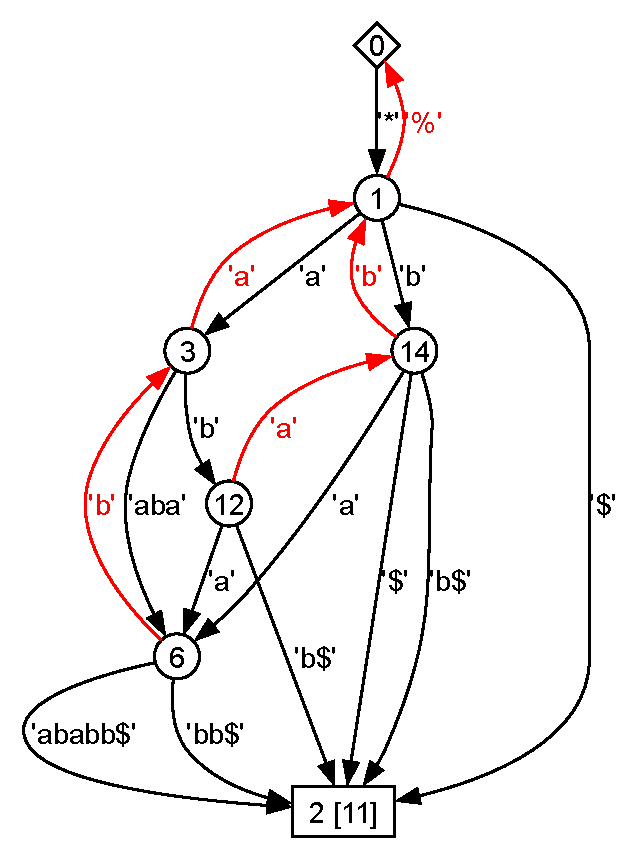
\includegraphics[height=.28\textwidth]{fig7.pdf}
%% \hfil
%% \includegraphics[height=.25\textwidth]{fig5.pdf}
%% \end{minipage}
%% \caption{The suffix tree, CDAWG, and a set of arrays 
%% for a text $T = aabaababb\daller$.}\label{fig:text:indexes}
%% \end{figure}
%% %%%%%%


%% \section{Modified Algorithms for MAW, MUS, and MRW}
%% \label{sec:mrw}

%We present modified algorithms for computing MAW, MUS, and MRW. 

% \subsection{A Generalization of MAWs, MUSs, and EBFs}
% \label{subsec:mf}
% Chen, Tsao, Deng, Wing-Kai, and Sadakane~\cite{chen2024taulambda} recently proposed the class $\MFO[k]$ of $k$-minimal factors.
% %In the following,
% We introduce the strict version of $k$-minimal factors.% 
% %%%%%
% \footnote{
% In the original definition, $W \in \MFO[k]$ if and only if 
% (i) $\Occ[](W) \le k$ and (ii) $\Occ[](U) > k$ for any proper superstring $U$ of $W$. Then, we see that $\MFO[k] = \bigcup_{0\le i\le k} \MF[k]$ holds for every $k\ge 0$. 
% }
% %%%%%
% For every $0\le k\le |T|$, a subword $W \in \Sub$ is a \textit{strict $k$-minimal factor} ($k$-MF, for short) of $T$ if
% (i) $\Occ[](W) = k$ and (ii) $\Occ[](U) > k$ for any proper superstring $U$ of $W$. 
% $\MF[k]$ denotes the set of all minimal factors in $T$. 
% %% \begin{lemma}
% We can show the next claim: for any subword $W = aYb \in \Sub$ with $|W|\ge 2$, where $a,b \in \Sigma,\; Y \in \Sigma^*$, (1) $W \in \MF[k]$ if and only if (2) $\Occ[](aYb) = k$, $\Occ[](aY) > k$, and $\Occ[](Yb) > k$ hold.
% Now, we give a uniform characterization of the classes of distinctive patterns. 
% %% \end{lemma}

% \begin{lemma}[classification of $\MAW, \MUS$, and $\EBF$]
%   For any factor $W \in \Sub$ with $|W|\ge 2$, the following conditions hold: 
%   \begin{enumerate}[(1)]
%   \item $W \in \MAW$ if and only if $W \in \MF[0]$. 
    
%   \item $W \in \MUS$ if and only if $W \in \MF[1]$. 
    
%   \item $W \in \EBF$ if and only if $W \in \bigcup_{k\ge 2}\MF[k]$. 
%   \end{enumerate}
% \end{lemma}

% %% \begin{lemma}[obsolute: characterization of MF]\label{lem:chara:ebf}
% %%   Let $k\ge 1$ be any integer, $G = \CDAWG$ be the CDAWG for a text $T$, and $W$ be any factor with $|W|\ge 2$, namely, $W = aYb \in \Sub$ with $Y \in \Sigma^*, a,b \in \Sigma$. Then, 
% %%   \begin{enumerate}[(1)]
% %%   \item $W \in \MF$, if and only if 
% %%   \item $\CDAWG(S)$ contains the nodes $x, y$, and $z$ such that: 
% %%     %satisfying the following conditions: 
% %%     \begin{itemize}
% %%     \item a node $x$ has the string label $\str(x) = aY$, is pointed by an $a$-Weiner link of $y$ that has an outgoing $b$-goto link pointing to $z$. 
% %%     \item a node $y$ with the string label $\str(y) = Y$ that has at least two Weiner links and at least two goto links. 
% %%     \item a node $z$ with $Yb$ as the prefix of its string label $\str(z)$ that is pointed by $y$ with outgoing $b$-edge, and has the weight $weight(z) = k$. 
% %%     \end{itemize}
% %%   \end{enumerate}
% %% \end{lemma}


%%% EOF
